%%%%%%%%%%%%%%%%%%%%%%%%%%%%%%%%%%%%%%%%%%%%%%%%%%%%%%%%%%%%%%%%%%%
%
% IMPERIAL COLLEGE LONDON DISSERTATION TEMPLATE 
%
%%%%%%%%%%%%%%%%%%%%%%%%%%%%%%%%%%%%%%%%%%%%%%%%%%%%%%%%%%%%%%%%%%%
%
% Copyright (c) 2008, Daniel Wagner, www.PrettyPrinting.net
% http://www.prettyprinting.net/imperial/
%%%%%%%%%%%%%%%%%%%%%%%%%%%%%%%%%%%%%%%%%%%%%%%%%%%%%%%%%%%%%%%%%%%

\documentclass[MSc,paper=a4,pagesize=auto]{icldt}
%\usepackage{showframe}
%\usepackage{cleveref} % lets us use chapter references
\usepackage{graphicx}  % lets us import graphics nicely

% Essential Setup
\title{Seeing the Big Data: Virtual Reality Visualisations of Large Datasets}
\author{Alexander Zawadzki (az2713)}
\date{September 2014}
\department{Computing}

% Optional
\supervisor{Professor Daniel Rueckert} 
\dedication{
My thanks to: 
\newline
\newline
Dr Paul Gass and Dr Ian Thompson, my bosses at Sharp Laboratories of Europe Ltd., for arranging for my funded sabbatical year at Imperial College London. 
\newline
\newline
Colleagues Dr Nathan Smith, Dr Graham Jones, Dr Jon Mather, and Dr Andrew Kay for sharing their passion for 3D display systems, and for bringing the strangest snack food back from business trips to Japan. Especial thanks to John Nonweiler, for setting an example of how development software \textit{should} be done.
\newline
\newline
Supporters Aashish Chaudhary at Kitware, and Brad Davis at ORIA for providing insight into VTK and the Oculus Rift SDK respectively.
\newline\
\newline
Friends in the MCS Program, in particular coffee-break-buddies Moritz Schrenk and Tereza Drskova. 
\newline
\newline
And last, but not least, I am indebted to my supervisors Professor Daniel Ruckert and Dr Bernhard Kainz. You have provided freedom when I wanted it, and guidance when I needed it. I am deeply grateful to you both. 
}

\begin{document}
\maketitle

\begin{abstract}
%\textbf{A Zawadzki, Department of Computing, Imperial College London}
%\\ \textbf{Abstract of Master's Thesis, submitted September 4th 2014}
%\\ \textbf{Seeing the Big Data: Virtual Reality Visualisations of Large Datasets}
A new pipeline is implemented for the visualisation of Human Connectome Project (HCP) data. HCP data are converted to an intermediate format, and then imported into the Visualisation Tool Kit (VTK). Through a series of extensions to the VTK pipeline, the data are rendered as distorted stereographic 3D images and output to an Oculus Rift virtual reality headset. Sensors on the headset track the user's head position and dynamically update the rendered image. The complete pipeline allows an immersive 3D display of data, with native access to all VTK functionality. A user study is conducted to evaluate the pipeline, and the resulting strengths and weaknesses are discussed.

%\hfill --- Alexander Zawadzki

\end{abstract}

\makededication
%\iffalse
\tableofcontents

\listoftables
\listoffigures

\chapter{Introduction}
\section{Context}
The growth of computing power and the volume of data available for analysis has far outpaced the development of visualisation hardware. In medical imaging multi-gigabyte datasets are common: as of June 2014 the Human Connectome Project has generated over 20 terrabytes of data on the three dimensional structure of the human brain. Courtesy of Moore's Law, the hardware available to process these data sets is growing exponentially. Display hardware has been constantly evolving. Unwieldy cathode-ray-tubes have morphed into slim LCSs less than one millimetre thick. Touch-screens became ubiquitous and tablet computers became commonplace. All of the dominant technologies share a common feature - they display 2D information for a user to look at. This situation may be set to change. 

Recent developments in virtual reality hardware offer a  paradigm shift in display technology. The change may see the popularity of displays that overlay information on top of the real world, so-called 'augmented reality', or displays that can provide a completely artificial 'virtual reality' experience. In either case, the displays will provide an immersive, three dimensional experience quite unlike any established technology today.

It is exhilarating and sometimes intimidating to be at the forefront of such a dynamic field. Since the project was initially planned, Oculus have significantly re-designed their Software Development Kit three times. In response to this, the ORIA project fundamentally revised their their book before it was even published. VTK continues to be developed and released on a daily basis, adding (and sometimes removing!) important features.

\section{Contributions}
This project has investigated the use of consumer grade virtual reality hardware, specifically the Oculus Rift DK1, as a tool for visualising and interacting with large datasets. The project has contributed to the open source community in a number of ways:

\begin{itemize}
  \item A plug-in was developed for Blender in order to allow the import of .vtk format data.
  \item The excellent Oculus Rift in Action (ORIA) project was forked on GitHub, at the suggestion of the project owner Brad Davis, to share bug-fixes with the community.
  \item Source code was ported from Paraview with encouragement from lead developer Aashish Chaudhary in order to bring Rift functionality to VTK.
  \item When relevant, assorted software problems were documented on Stack Overflow in 'Question and Answer' format. The response to these posts has been very positive, bumping my account "\textit{GnomeDePlume}" to the top 24\% of contributors in 2014.  
\end{itemize}

In comparison to the size and scope of these established projects, this project has made only incremental contributions. Nevertheless, these contributions have been contributed in the spirit of open source collaboration and have have incrementally advanced the state-of-the-art.

The academic impact of this project is more difficult to quantify. TODO: suggestions welcome! Virtual reality hardware is not widely available, although the sudden success of the Microsoft Kinect has highlighted the explosive adoption of new technology into research when available at commodity prices.

\newpage
\section{Structure of the Report}
As the project dealt with implementing a pipeline, it seems natural for the report to follow the process from raw data acquisition to the final display image.

Following this logic, Chapter~2 discusses the how the Human Connectome Project (HCP) maps the structure of the brain using DTI and fMRI imaging. This is important because the nature of the raw data affects all subsequent stages in the pipeline. Chapter~3 discusses the HCP data structure, and how it may be converted to intermediate formats. Chapter~4 shows how a Visualisation Tool Kit (VTK) pipeline can be constructed and HCP data can be processed for interaction and display on a standard 2D computer monitor. 

Chapter~5 breaks from the sequential structure in order to introduce the Oculus Rift hardware, and shows how the collimating optics in the headset will distort images unless extra distortion shaders are used. The report then returns to the VTK pipeline in Chapter~6 to discuss the good, the bad and the ugly ways to apply shaders so that images can be rendered correctly to the Rift. 

\begin{figure}[h]
    \centering
    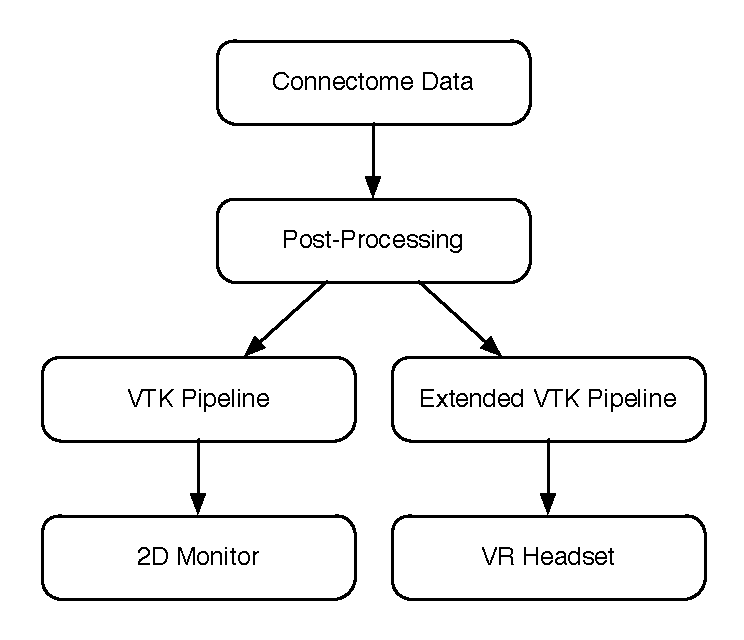
\includegraphics[scale=0.5]{resources/data_pipeline_overview}
    \caption{The Full Pipeline}
    \label{fig:the_full_pipeline}
\end{figure}


With a complete pipeline, Chapter~7 discusses how the system was evaluated. This evaluation identified numerous strengths and weaknesses, and suggestions for further work are explored.

Finally, Chapter~8 concludes by synthesizing findings from each stage in the project, and reviewing the most interesting learning outcomes.

\chapter{Connectome Data}
\section{This Is Your Brain}
\section{This Is Your Brain on DTI-MRI}
\section{HCP Data}

\chapter{Post-Processing}
\section{Choosing an Intermediate Format}
\section{Importing Data to Blender}
\section{Mesh Analysis and Simplification}

\chapter{The Visualisation Tool Kit}
\section{An Overview of the VTK Pipeline}
\section{Basic Actor Manipulation}
\section{Advanced Visualisation Tools}

\chapter{Displaying Images on the Rift DK1}
\section{Introducing the Rift DK1}
\section{Collimating Optics and Software Compensation}
\section{Integrated Sensors and the HMD}

\chapter{Extending VTK}
\section{The Need for Shaders}
\section{Applying GLSL Shaders to Materials}
\section{Applying GLSL Shaders to Objects}
\section{Applying GLSL Shaders to Buffers}
\section{Porting and Sub-Classing}

\chapter{Results}
\section{Automated Testing with CTest}
\section{Hardware Limitations}
\section{Software Limitations}
\section{Human Factors}

\chapter{Conclusion}
\cite{Nobody06}

\bibliography{bibtex/mybib}
\bibliographystyle{plain}


\end{document}